%
% CERN REPORT template for LaTeX
%
% Public version 1.0
% 2018-2019  Vasileios S.Dimakopoulos
%
% THIS IS THE MAIN FILE  (i.e. compile this file, compiling the others directly won't work)
%
\documentclass[a4paper,10pt,twoside]{report}

%all the other includes etc. are done in the thesis.sty file.
\usepackage{thesis}
\usepackage[noframe]{showframe}% http://ctan.org/pkg/showframe
\providecommand*\LenToUnit[1]{#1\@gobble}
\usepackage{helvet}
\renewcommand{\familydefault}{\sfdefault}
\newcommand\AtPageUpperRight[1]{\AtPageUpperLeft{
\put(\LenToUnit{0.9\paperwidth},\LenToUnit{-1cm}){#1}}
}


%\usepackage[margin=0.3in]{geometry}
\AddToShipoutPictureBG*{
  \AtPageUpperLeft{\raisebox{-\height}{
\includegraphics[width=4in]{figures/openlab_pic}}}%
}

\AddToShipoutPictureBG{
 \ifnum\value{page}>1
 \AtPageUpperRight{\raisebox{-\height}{
\includegraphics[scale=0.25]{figures/openlab_logo}}}
 \fi
}

%
%
% These commands need to be defined in order to produce a correct and personalized document
%
\newcommand{\doctitle}{Employing HPC for Heterogeneous HEP Data Processing}
\newcommand{\footerTitle}{DEEP-EST}
\newcommand{\me}{Marco Barbone} %Long name problems \\ looked silly on one line
\newcommand{\keywords}{keyword1, keyword2, keyword3}
\newcommand{\version}{}
\newcommand{\monthYear}{\today}



\newcommand{\firstCommitteeMember}{Viktor Khristenko}
\newcommand{\secondCommitteeMember}{Felice Pantaleo}
\newcommand{\thirdCommitteeMember}{Maria Girone}

\author{\me}

%Your Cern deparment and/or other affiliation
\newcommand{\department}{CERN IT-DI-OPL \\ DEEP-EST}



%
% PDF settings
%
\hypersetup
{
    pdfauthor={\me},
    pdftitle={\doctitle},
    pdfsubject={\doctitle},
    pdfkeywords={\keywords}
}
\cfoot{\vspace{0.1in}
\includegraphics[width=1.1\linewidth]{figures/openlab_banner}}
%To change the "name of the report go to thesis.sty and change fancyfoot[L]

\newcommand{\nocontentsline}[3]{}
\newcommand{\tocless}[2]{\bgroup\let\addcontentsline=\nocontentsline#1{#2}\egroup}

\usepackage[
singlelinecheck=false % <-- important
]{caption}
\usepackage{algorithm}
\usepackage[noend]{algpseudocode}
\usepackage{amssymb}

\let\oldemptyset\emptyset
\let\emptyset\varnothing

\newenvironment{claim}[1]{\par\noindent\underline{Claim:}\space#1}{}
\newcommand{\norm}[1]{\left\lVert#1\right\rVert}

% \graphicspath{{img}
% \usepackage{graphicx}

% \usepackage{tgbonum}
\usepackage{lineno}
\begin{document}
\linenumbers
% \fontfamily{qcr}

%use this include for PDF and distribution versions
\pagenumbering{roman}

\begin{titlepage}
\begin{center}

%\vspace{-0.85cm}
\large
%\vspace*{10cm}

\setlength{\TPHorizModule}{1mm}
\setlength{\TPVertModule}{\TPHorizModule}
% Set the Paragraph Indent to zero, so the first line is not Indented
% Back-up the current value so it can be put back at the end of the title page
\newlength{\backupparindent}
\setlength{\backupparindent}{\parindent}
\setlength{\parindent}{0mm}			
% Begins a textbox at 30 mm from the left of the edge of the paper and 89 mm from the top
% The width of the textbox is 150 mm 
% The height of the box cannot be defined, so it is your task to keep the text not too long
\begin{textblock}{150}(30,50)
    \vspace*{15mm}
    \Huge
    \vspace{4cm}
    \textcolor{OpenlabBlue}{\textbf{\doctitle }}\\
    \Large
    \vspace*{5mm}


    \begin{flushleft}
        \textcolor{OpenlabDarkBlue}{\textsc{August 2018}}\\
        \large
	
    \end{flushleft}
    \vspace*{1in}
    \begin{figure}
        \raggedleft
    \begin{minipage}[r]{0.2 \textwidth} %scale number here too move the Author and Supervisor section
   \begin{flushleft}                     % Larger number means further left on the page and vice versa.
	\textsc{\textbf{Author:}}\\
    \me\\\bigskip\bigskip

   % \small
   \normalsize
    \department\\\bigskip\bigskip
    
    \textsc{\textbf{Supervisors:}}\\\medskip
	%\begin{tabular}{ccc}
    \firstCommitteeMember\\
    \secondCommitteeMember\\
%    \thirdCommitteeMember\\
	%\end{tabular}
   \end{flushleft}

\end{minipage}    
\end{figure}
\end{textblock}


\vspace*{20mm}


\vfill
\version

\vfill
%\docdate
\large

\includegraphics[scale=0.095]{figures/openlab}
% Put the Paragraph Indent back to its original value
\setlength{\parindent}{\backupparindent}
\end{center}
\end{titlepage} 

\normalsize

\newpage

\chapter*{\textcolor{OpenlabDarkBlue}{Project Specification} }\label{chapter:specification}
project specification

\chapter*{\textcolor{OpenlabDarkBlue}{Abstract}} \label{chapter:abstract}
THIS IS MY ABSTRACT

\begingroup
\color{OpenlabDarkBlue}
\tableofcontents
\endgroup

\listoffigures

\listoftables

\lstlistoflistings


\clearpage

\setcounter{page}{10}
\pagenumbering{arabic}
\chapter{From physics to... Physics}\label{chapter:01}
\begin{figure}[ht]
  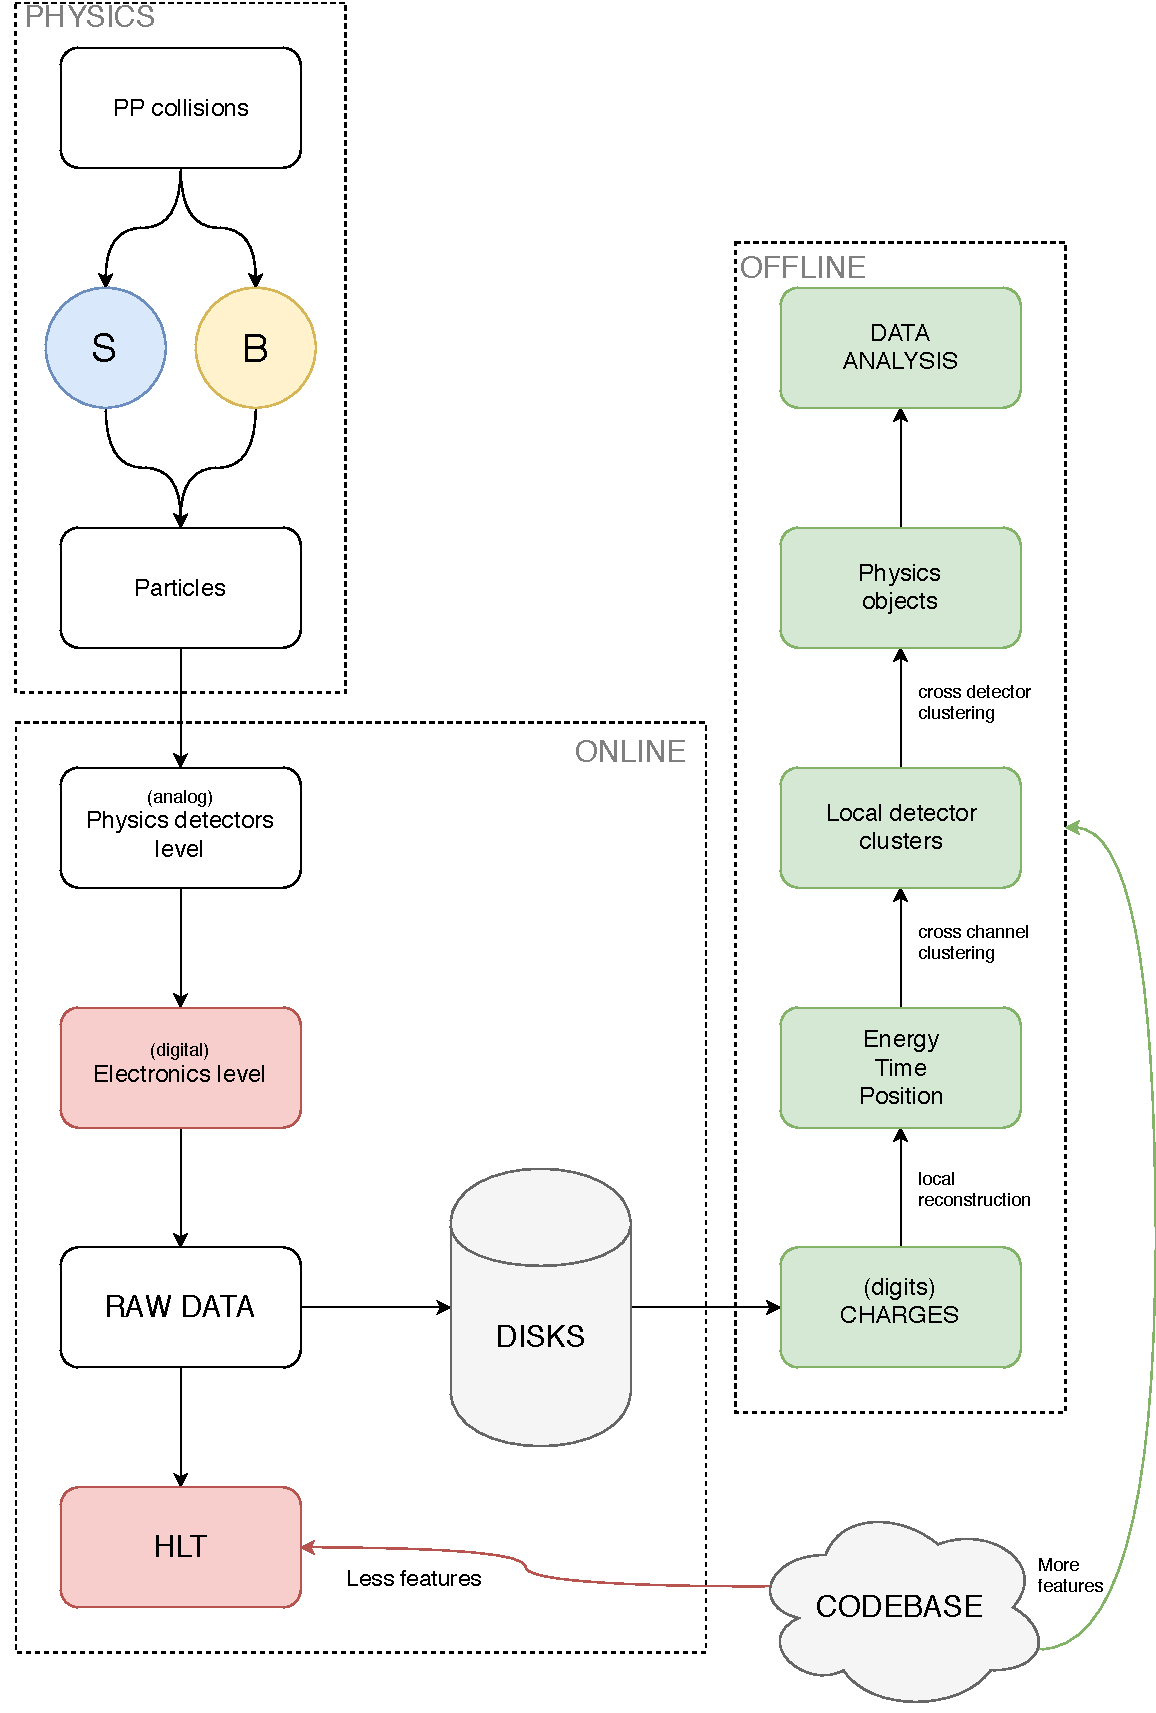
\includegraphics[height=\textheight]{img/dataflow}
  \caption{Cern data flow from collisions to analysis}
  \label{img:dataflow}
\end{figure}
% This might be an introduction
Modern high energy physics (HEP) requires analysis. To make it possible several large scale objects are needed: from accelerators, detectors, data centers to the thousands of people involved to design and run the infrastructure. Here at CERN everything starts with physics by colliding particles and everything ends with the physics performed by analyzing the data acquired. But, to produce the necessary data, in the right amount, a long and complicated process, showed in figure \ref{img:dataflow}, is involved. It is worth to briefly describe it to understand the reason of our work and where is it place inside it. \\
\paragraph{Data generation}
The process starts with \textbf{particle collisions} this lead to particle interactions that create some \textbf{intermediate product}. This intermediate product can not be directly observed, bit it decays in \textbf{particles} that go through the detectors. The intermediate product is divided in \textbf{X} and \textbf{Y}, X is what physicists are trying to study while Y is something that produces similar particles as Y but is not what they are looking for.
\paragraph{Data aquisition}
Detectors are split in two levels: \textbf{physics detector level} and \textbf{electronics level}. The physics level takes in input sensor readouts and produces an analog signal. This analog signal is the digitalized by the electronics level. This level also decides if the event is interesting or not, based on this the event is discarded or recorded. 
% Should I say that not interesting reading are discarded here?
The event that survive this ends up dumped into \textbf{disks} and send to the \textbf{High level trigger}. \\
It is important to notice that these decision are taken in real time, to meet the throughput and timing requirements everything is built with \textbf{asic}s and \textbf{fpga}s boards. 
\paragraph{Data processing} 
Data processing is performed both online and offline. %The \textbf{high level trigger} (HLT) performs it online while all the rest is offline. 
The first step, called \textbf{local reconstruction}, in the offline data processing is to transform charges in physical quantities such as \textbf{energy}, \textbf{time}, and \textbf{position}. This operation is done channel by channel independently form each other. Then, information coming from different channel of the same detector are combined by the \textbf{cross channel clustering} into \textbf{local detector cluster}s. The final step needed to obtain \textbf{particle object}s is the \textbf{cross detector clustering} in which data coming from different detector is combined. The particle object forms the dataset used by theoretical physicists to do physics. \\
\paragraph{High level trigger (HLT)}
The \textbf{HLT} belongs both to data acquisition and data processing, since it would not be correct to include it in one of this categories, it deserves a separate discussion. \\
The HLT main purpose is to select interesting events before writing them to disk. In order to accomplish this, it runs the same code used for the offline processing, but \textbf{online} and with less features because of strict time constraints. \\
The main difference between \textbf{L1} and HLT is that L1 is implemented in hardware with no host while HLT is software based, it runs on hosts with accelerators used to speed-up the processing.


\chapter{Local energy reconstruction}\label{chapter:02}
The HLT shares the same code used for offline data processing, thus the processing pipeline is more or less the same. The fundamental difference is that the output is used to perform event classification instead of data analysis. 
\begin{figure}[ht]
  \centering
  \caption{HLT processing pipeline}
  \label{img:hlt}
  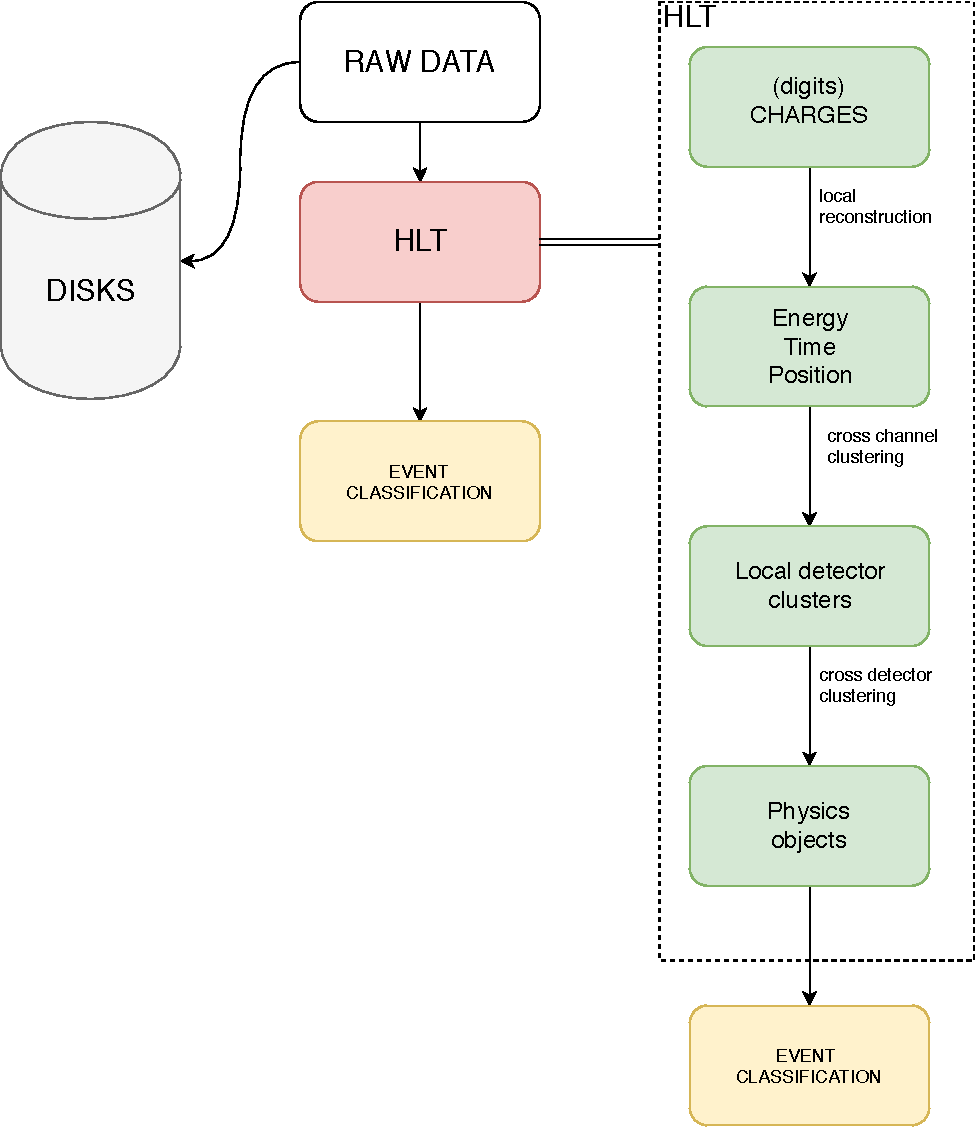
\includegraphics[width=.75\textwidth]{img/hlt}
\end{figure}
The table \ref{table:timeshare} shows how much time is spent in every single step of the reconstruction process. Most of it is spent into tracking but after it, the second more time consuming step is HCAL+ECAL local reconstruction that takes $113 ms$ corresponding to $24\%$ of the total time.
\begin{figure}[ht]
  % \centering
  \caption{Data processing time share}
  \label{img:hlt}
  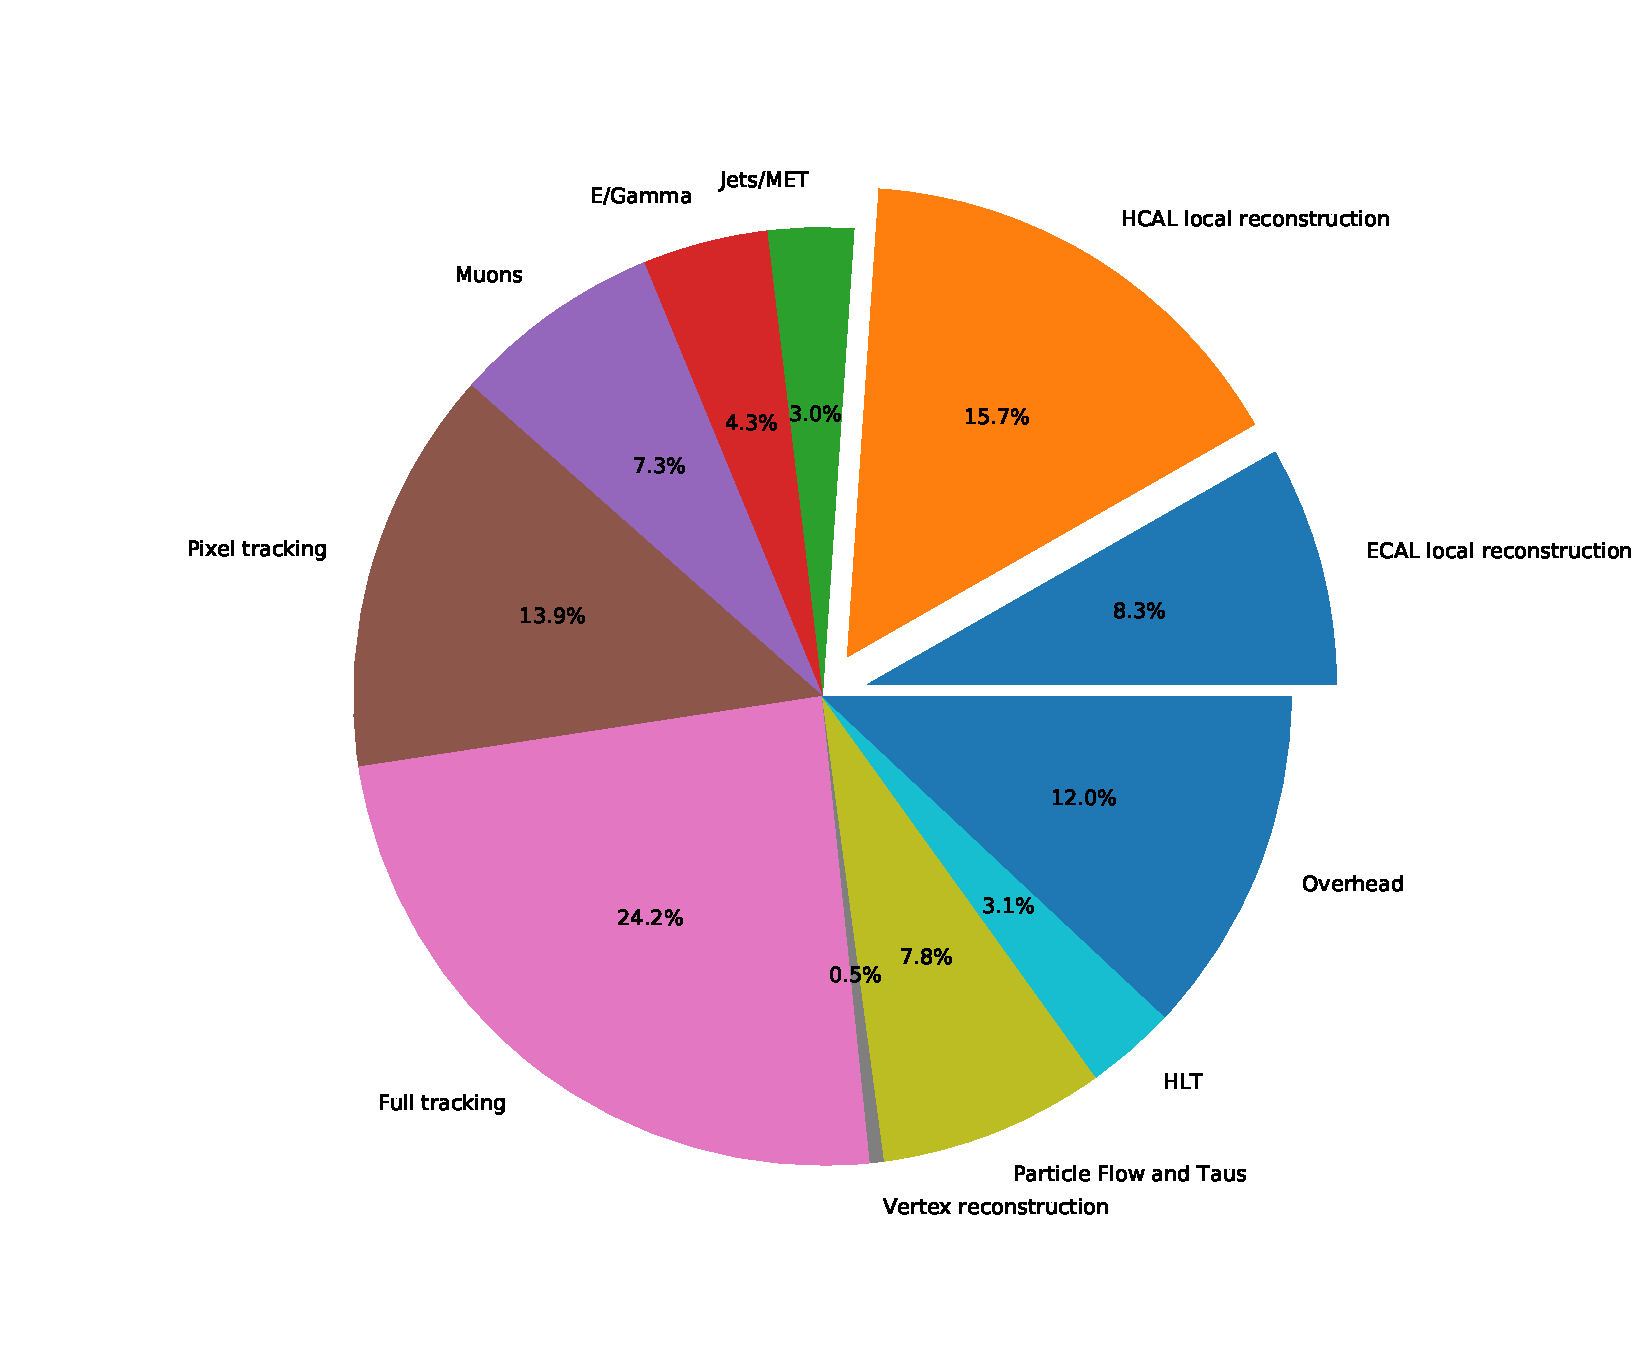
\includegraphics[width=\textwidth]{img/timeshare}
\end{figure}
Given the time needed to perform this reconstruction even achieving a speedup of two would reduce the total processing time of more than $10\%$. This is my focus in this project try to reduce it as much as possible.
\begin{table}[ht]
  \caption{Time spent into the various HLT reconstruction steps}
  \label{table:timeshare}
  \begin{tabular}{lll}
    \hline
    Step                      & Real-Time      & Percentage \\ \hline
    ECAL local reconstruction & 38.9 ms        & 8.25\%     \\
    HCAL local reconstruction & 73.9 ms        & 15.67\%    \\
    Jets/MET                  & 14 ms          & 2.97\%     \\
    E/Gamma                   & 20.4 ms        & 4.33\%     \\
    Muons                     & 34.2 ms        & 7.25\%     \\
    Pixel tracking            & 65.7 ms        & 13.93\%    \\
    Full tracking             & 114.2 ms       & 24.22\%    \\
    Vertex reconstruction     & 2.3 ms         & 0.49\%     \\
    Particle Flow and Taus    & 36.8 ms        & 7.8\%      \\
    HLT                       & 14.7 ms        & 3.12\%     \\
    Overhead                  & 56.4 ms        & 11.96\%    \\
    Total                     & 471.5 ms       & 100\%      \\ \hline
  \end{tabular}
\end{table}
\section{Problem statement}
As the name says the goal of this step is: \\
\begin{claim}
  For each channel \{given $n$ charge readouts $\rightarrow$ reconstruct the energy\}. \\
  \quad Where in this case $n$ is fixed to 10. 
\end{claim}\\
Translated into mathematical terms this means:
\begin{equation}\label{eq:chisq}
  \begin{split}
    & \min(\chi^2)=\min(\norm{Px - b}) \\
    & \forall x: x \geq 0\\
    \text{where:}&  \\
    & x = \text{energy vector} \\
    & P:CHARGE \rightarrow ENERGY =\text{feature matrix} \\
    & b = \text{charge vector}
  \end{split}
\end{equation}
Which is a min$\chi^2$ problem with additional positivity constraints. This constraint is present because physically speaking negative energy does not make sense. \\
As shown in \cite{amplituamplitude_reconde_recon} the statement above is incomplete. A perfect mapping from charges to energy does not exist because signal from the shower does not dissipate within one time slice ($25ns$). Adding the correlation term this problem becomes:
\begin{equation}\label{eq:constrained_chi_sq}
  \begin{split}
      &\min(\norm{(Px - b)^T\Sigma(x)^{-1}(Px - b)}) \\
      & \forall x: x \geq 0\\
  \end{split}
\end{equation}
It is worth pointing out that $\Sigma$ depends on x, meaning also $\Sigma$ is unknown. \\
To compute $\Sigma$ an iterative procedure is used:
\begin{enumerate}
  \item Compute $\Sigma$.
  \item Minimize $\chi^2$.
  \item If not convergence goto 1.
\end{enumerate}
More precisely $\Sigma$ is the covariance matrix representing the noise correlation between time samples i and j, obtained from data where no signal is present, and the single sample noise.\\
To solve the problem stated in \ref{eq:chisq} several algorithms exists, for example \textbf{lsqnonneg} illustrated in \cite{nnls} and the \textbf{ffnls} illustrated in \cite{fnnls}. The one implemented is fnnls since as measured in \cite{Chen09nonnegativityconstraints} it is faster.\\
The problem presented in \ref{eq:constrained_chi_sq} is not a $\chi^2$ problem but to solve it with nnls needs to be reduced into the canonical form. The redution exploits the Cholesky decomposition and is illustrated in \ref{eq:reduction}.
\begin{equation}\label{eq:reduction}
  \begin{split}
  & (Px-b)^T\Sigma(x)^-1(Px-b)\\
  \equiv &\quad \Sigma=LL^T,\space (AB)^{-1} = B^{-1} A^{-1}\\
  & (Px-b)^T L^{-T} L^{-1} (Px-b)\\
  \equiv &\quad (AB)^T = B^T A^T \\
  & (L^{-1}Px-L^{-1}b)^T  L^{-1} (Px-b)\\
  \equiv & \\
  & (L^{-1}Px-L^{-1}b)^T (L^{-1}Px-L^{-1}b)\\
  \equiv &\quad L^{-1}P=P', \space L^{-1}b=b' \\
  & (P'x-b')^T(P'x-b')\\
  \equiv & \\
  & min(\chi^2)
  \end{split}
\end{equation}

\section{Fast non negative least square (FNNLS)}


\chapter{Conclusions}\label{chapter:conclusions}
From our analysis is it possible to conclude that GPUs outperforms CPUs in HEP workflows. In all tests we did not manage to generate enough threads to fill all the warps. And even in this case the speedup showed in table \ref{tab:speedup} is of a factor of $2.67$. Also, the CPU implementation optimized with all the numerical, algorithmic, and architecture dependent tweaks reaches a speedup of $1.38$.  
\begin{table}[h]
  \caption{Speedup achieved after optimizing the matrix multiplication.}
  \label{tab:speedup}
\begin{tabular}{lrrrrrrr}
\toprule
channels &  1024  &  2048  &  4096  &  8192  &  16384 &  32768 &  65536 \\
\midrule
legacy\_multifit\_cpu &   1.00 &   1.00 &   1.00 &   1.00 &   1.00 &   1.00 &   1.00 \\
legacy\_multifit\_gpu &   0.62 &   1.22 &   1.77 &   2.09 &   1.89 &   2.10 &   2.23 \\
multifit\_cpu        &   1.25 &   1.38 &   1.35 &   1.35 &   1.33 &   1.34 &   1.34 \\
multifit\_gpu        &   0.96 &   1.57 &   2.09 &   2.56 &   2.31 &   2.54 &   2.67 \\
multifit\_gpu\_swap   &   0.42 &   0.73 &   1.10 &   1.15 &   1.11 &   1.21 &   1.23 \\
multifit\_cpu\_swap   &   0.45 &   0.48 &   0.51 &   0.50 &   0.50 &   0.50 &   0.50 \\
\bottomrule
\end{tabular}
\end{table}


%Choose a good bibliography style, plain would do often, but these might be nice too
%\bibliographystyle{these}
\bibliographystyle{plain}
\bibliography{references.bib}

\clearpage %ensures the Appendix ToC entry points to the correct appendix page
\appendix
\addcontentsline{toc}{chapter}{Appendix} %add line to mark start of appendixes, 

\chapter{My First Appendix}
In this file (appendices/main.tex) you can add appendix chapters, just as you did in the thesis.tex file for the `normal' chapters.
You can also choose to include everything in this single file, whatever you prefer.

\end{document}
